%!TEX root = ../MainBody.tex

\chapter{求解器场景编辑与仿真任务管理系统}
\label{chap:gui}

\section{引言}
\label{sec:gui:intro}

经过第三章和第四章的工作，Stardis 求解器已具备基于 Wavefront 架构的并行化路径追踪求解能力与 OptiX GPU 硬件光追查询后端，能够以 CPU-GPU 混合架构高效处理辐射、传导、对流三类耦合热输运场景。然而，高效的求解算法只是仿真工作流的核心环节之一——将算法能力转化为可重复、低门槛的工程实践，同样需要系统性的工具链支撑。

Stardis 求解器以 \texttt{stardis-input} 领域描述语言（Domain-Specific Language, DSL）\cite{mesostarStardisinputThermalSystem2024}作为唯一的场景输入格式。该 DSL 以关键字驱动的逐行 ASCII 文本定义热输运系统的全部要素——介质体、边界条件、连接关系、外部辐射环境等，并具有完整的 BNF 形式文法规范。然而，该 DSL 的纯文本编辑方式在实际仿真工作流中存在若干系统性使用障碍：

（a）位置参数无标签。DSL 的具体语法采用严格位置编码，典型行如 \texttt{SOLID body0 1.5 2700.0 900.0 AUTO 300.0 UNKNOWN 0.0 BOTH body0.stl}，含 10 个位置参数，含义须对照文法规范逐项核对。参数项繁多、顺序固定，手动编辑极易出错，且错误只能在求解器执行时才能被察觉。

（b）几何信息不可见。DSL 描述中几何体仅以 STL 文件路径引用，空间关系、法线朝向和表面分区完全无法从文本推断。几何定义错误（如法线翻转、区域遗漏）只能在求解器产出异常结果后才能发现。

（c）表面区域划分依赖外部工具。DSL 的 $\langle\text{boundary-condition}\rangle$ 产生式要求每条边界条件显式引用一组 STL 文件，将同一几何体拆分为多个换热参数不同的子区域时，须提前在三维建模软件中按区域切割 STL 并分别导出——DSL 自身不具备交互式表面分区能力。

（d）仿真任务参数组装繁琐。Stardis CLI 接受数十个运行参数（\texttt{-M}、\texttt{-n}、\texttt{-t}、\texttt{-V}、\texttt{-R}、\texttt{-p}、\texttt{-P} 等），其中 IR 渲染的 \texttt{-R} 参数需将摄像机姿态全部内联为字符串；后处理工具 HTPP 亦有独立参数体系。这些运行时参数不属于 \texttt{stardis-input} DSL 的定义范围，多组参数实验的命令行拼接容易遗漏字段。

（e）多任务批量执行无自动化。多帧时序仿真或探针计算与 IR 渲染的组合实验需按序执行多组任务并自动触发后处理，手动监控进度、处理中间错误代价高。

本章设计并实现 GUI 场景编辑器 StardisEditor，以 Python 3 + PyQt5 + VTK 技术栈为 \texttt{stardis-input} DSL 构建可视化编辑环境。编辑器以 DSL 的形式文法为解析与写出的基础，同时在 DSL 表达能力之外提供三项关键扩展：三维可视化预览场景几何、交互式画笔标注表面区域、图形化配置与队列化执行仿真任务。

本章内容组织如下：\ref{sec:gui:dsl} 概述 \texttt{stardis-input} DSL 的文法结构与纯文本编辑局限性；\ref{sec:gui:architecture} 提出系统架构设计；\ref{sec:gui:modules} 详述功能模块的设计与实现；\ref{sec:gui:cases} 通过应用案例展示完整工作流；\ref{sec:gui:summary} 总结本章贡献。


%% ============================================================
\section{\texttt{stardis-input} 场景描述语言}
\label{sec:gui:dsl}

\subsection{文法概述}

Stardis 求解器的场景输入格式 \texttt{stardis-input}\cite{mesostarStardisinputThermalSystem2024} 是一种面向耦合热输运系统描述的文本 DSL，其文法以 BNF（巴科斯-诺尔范式）产生式定义。顶层结构为：
%
\begin{equation}
\langle\text{thermal-system}\rangle ::= \langle\text{description-line}\rangle\ldots
\label{eq:gui:bnf-top}
\end{equation}
%
每条描述行（description-line）为以下六类之一：
%
\begin{equation}
\begin{aligned}
\langle\text{description-line}\rangle ::=\ &\langle\text{medium}\rangle \mid
  \langle\text{connection}\rangle \mid
  \langle\text{boundary-condition}\rangle \\
  &\mid\ \langle\text{scaling}\rangle \mid
  \langle\text{program}\rangle \mid
  \langle\text{comment}\rangle
\end{aligned}
\label{eq:gui:bnf-line}
\end{equation}
%

其中，$\langle\text{medium}\rangle$ 描述固体或流体介质及其热物性参数；$\langle\text{boundary-condition}\rangle$ 描述施加在介质表面的温度（Dirichlet）、对流（Robin）、热流（Neumann）或混合边界条件；$\langle\text{connection}\rangle$ 描述两个介质之间的固-流或固-固接触关系。各类描述行的展开式进一步规定了参数顺序和类型约束，例如固体介质的产生式为：
%
\begin{equation}
\begin{aligned}
\langle\text{solid-const}\rangle ::=\ &\texttt{SOLID}\ \langle\text{medium-name}\rangle\ \langle\lambda\rangle\ \langle\rho\rangle\ \langle c_p\rangle \\
  &\langle\delta\rangle\ \langle T_{\rm init}\rangle\ \langle T_{\rm imposed}\rangle\ \langle P_{\rm vol}\rangle \\
  &\langle\text{triangle-sides}\rangle\ldots
\end{aligned}
\label{eq:gui:bnf-solid}
\end{equation}
%
其中 $\langle\delta\rangle ::= \texttt{AUTO} \mid \text{real}$，$\langle T_{\rm imposed}\rangle ::= \texttt{UNKNOWN} \mid \text{real}$。类似地，Robin 型边界条件的产生式为：
%
\begin{equation}
\begin{aligned}
\langle\text{robin-solid-const}\rangle ::=\ &\texttt{H\_BOUNDARY\_FOR\_SOLID}\ \langle\text{bound-name}\rangle \\
  &\langle T_{\rm ref}\rangle\ \langle\varepsilon\rangle\ \langle f_s\rangle\ \langle h_c\rangle\ \langle T_{\rm env}\rangle\ \langle\text{triangles}\rangle\ldots
\end{aligned}
\label{eq:gui:bnf-robin}
\end{equation}
%
所有物理量采用国际单位制。几何数据通过 $\langle\text{triangles}\rangle ::= \langle\text{stl-path}\rangle$ 以外部 STL 文件路径引用。

\subsection{语义约束}

除语法层面的产生式外，\texttt{stardis-input} 还包含若干不可由 BNF 表达的语义约束：
\begin{itemize}
  \item 包壳唯一性（enclosure constraint）：每个包壳（enclosure）的全部构成面必须由单条描述行定义，不可跨行拆分，以保证系统中的每个密闭空间由单一介质构成；
  \item 边界归属：每条 $\langle\text{boundary-condition}\rangle$ 所引用的 STL 面片集必须几何上属于某个 $\langle\text{medium}\rangle$ 的表面——此归属关系在 DSL 文本中是隐式的，由求解器在加载时通过几何匹配确定；
  \item 名称唯一性：所有描述名称（介质名、边界名、连接名）全局唯一，大小写敏感，且不得与文法关键字重名；
  \item 几何侧约定：$\langle\text{side-specifier}\rangle ::= \texttt{FRONT} \mid \texttt{BACK} \mid \texttt{BOTH}$，其中 \texttt{BACK} 为三角面法线（右手法则）指出的一侧——封闭几何体法线朝外时，应使用 \texttt{FRONT} 描述包围介质。
\end{itemize}

\subsection{纯文本编辑的局限性}

\texttt{stardis-input} DSL 的文法设计面向求解器的批处理解析，而非面向人工交互编辑。其位置参数语法使得编辑时必须对照文法规范逐字段定位；产生式 $\langle\text{triangles}\rangle$ 仅支持引用外部 STL 文件路径、不允许内联几何定义，因此表面区域的划分必须借助外部建模工具预先完成；边界到介质的归属关系在文本中完全隐式，多介质场景下手动维护容易出错。

这些局限性构成了本章工作的出发点：为 \texttt{stardis-input} DSL 构建一个可视化编辑器，在 DSL 的形式文法基础上提供语法感知的解析与写出，同时在 DSL 的表达能力之外扩展交互式几何预览、表面区域标注和仿真任务管理功能。

%% ============================================================
\section{系统架构设计}
\label{sec:gui:architecture}

\subsection{设计思路}

StardisEditor 的核心数据流可概括为：
%
\begin{quote}
\texttt{stardis-input} 具体语法 $\xrightarrow{\text{解析}}$ 语义模型 $\xrightarrow{\text{可视化投射}}$ 多面板交互编辑 $\xrightarrow{\text{序列化}}$ \texttt{stardis-input} 具体语法
\end{quote}
%
其中，DSL 文本与语义模型之间的往返转换由解析/写出工具完成：\texttt{SceneParser} 按 DSL 文法将文本解析为内存中的语义模型 \texttt{SceneModel}，\texttt{SceneWriter} 将模型序列化回合法的 DSL 文本。交互界面的三个展示组件（场景树、3D 视口、属性面板）以不同形式投射同一份语义模型，用户编辑直接作用于 \texttt{SceneModel}，而不直接参与 DSL 文本的序列化过程。此数据流决定了系统的两个核心架构约束：（1）需要 Model-View 分离以保证三个投射面板的数据一致性；（2）解析器和写出器必须严格遵循 DSL 文法，保证往返（round-trip）正确性。

为此，本文采用 Model-View 架构配合 PyQt5 信号/槽机制实现解耦：\texttt{SceneModel} 作为单一数据源；各展示组件持有 \texttt{SceneModel} 引用并从中读取数据；用户修改通过 \texttt{SceneEditor}（主窗口，组件编排器）的信号/槽链路写回模型并触发其余组件刷新。

\subsection{模块划分}

系统按职责自顶向下分为三个层次，如表~\ref{tab:gui:modules} 所示。

\begin{table}[htbp]
  \centering
  \bicaption{StardisEditor 模块层次划分}{StardisEditor module hierarchy}
  \label{tab:gui:modules}
  \footnotesize
  \begin{tabular}{p{2cm}p{5.2cm}p{5.8cm}}
    \toprule
    层次 & 主要类 & 职责 \\
    \midrule
    交互层 & \texttt{SceneEditor}、\texttt{SceneTreePanel}、\texttt{PropertyPanel}、\texttt{SceneViewport}、\texttt{SurfacePainter} & 主窗口编排、层级树/属性面板/3D 视口投射、交互式画笔标注 \\
    数据模型层 & \texttt{SceneModel}、Task 数据对象（\texttt{Camera}、\texttt{Probe} 等）、任务队列 & DSL 语义模型（Python \texttt{dataclasses}）、仿真任务与观测数据、队列调度状态 \\
    工具层 & \texttt{SceneParser}、\texttt{SceneWriter}、\texttt{CommandBuilder}、\texttt{TaskRunner} & DSL 具体语法 $\leftrightarrow$ 语义模型双向转换、CLI 参数组装、子进程执行 \\
    \bottomrule
  \end{tabular}
\end{table}

交互层的各面板组件通过信号/槽机制读写数据模型层的 \texttt{SceneModel}，不直接接触 DSL 文本的序列化。DSL 文本与语义模型之间的往返转换由工具层的 \texttt{SceneParser} 和 \texttt{SceneWriter} 完成；仿真任务的 CLI 参数组装与子进程执行同样由工具层的 \texttt{CommandBuilder} 和 \texttt{TaskRunner} 负责。图~\ref{fig:gui:architecture} 展示了系统的三层架构及层间依赖关系。

\begin{figure}[htbp]
  \centering
  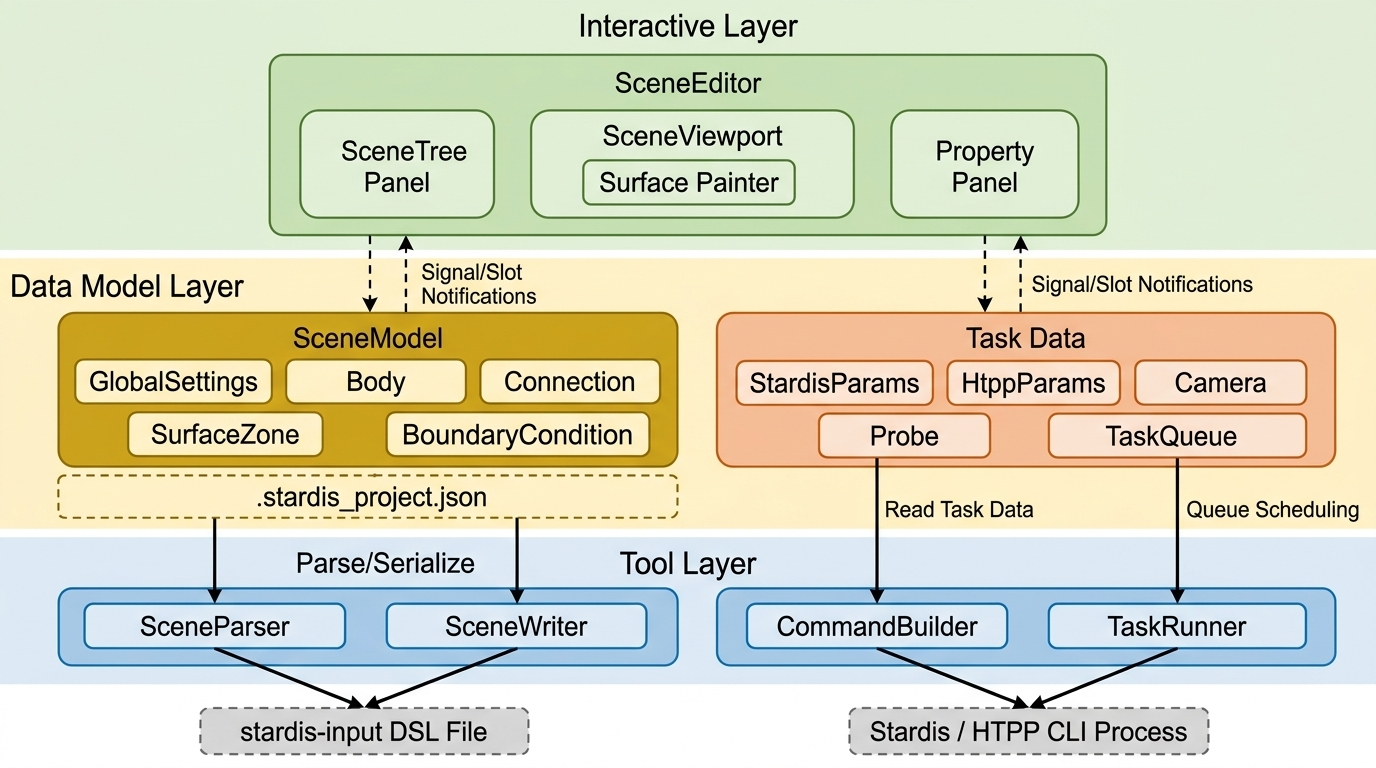
\includegraphics[width=0.9\textwidth]{Figures/editor/architecture/架构.jpg}
  \bicaption{StardisEditor 系统层级架构}{StardisEditor system layer architecture}
  \label{fig:gui:architecture}
\end{figure}

\subsection{工程文件}

编辑器以独立工程文件（\texttt{.stardis\_project.json}）持久化 DSL 之外的编辑器状态：表面区域到介质体的归属映射、区域序号池、画笔标注的面片集、探针/摄像机/灯光位姿、任务队列配置和编辑器版本号。工程文件与 DSL 场景文件共同构成完整的工程描述，支持一键恢复上次工作状态。


%% ============================================================
\section{功能模块设计与实现}
\label{sec:gui:modules}

\subsection{DSL 解析与写出}
\label{sec:gui:parser}

本模块实现 \texttt{stardis-input} DSL 具体语法与内存语义模型 \texttt{SceneModel} 之间的双向转换，是系统全部功能的数据基础。

\subsubsection{语义模型}

\texttt{SceneModel} 是 DSL 的抽象语义表示。其类层次直接对应 DSL 文法中的产生式类别：根对象持有 \texttt{GlobalSettings}（对应 $\langle\text{scaling}\rangle$ 和 $\langle\text{rad-env}\rangle$）、\texttt{Body} 列表（对应 $\langle\text{medium}\rangle$）、\texttt{Connection} 列表（对应 $\langle\text{connection}\rangle$）。每个 \texttt{Body} 下挂载 \texttt{SurfaceZone} 列表，其边界条件对象按 DSL 文法分为四种子类，与 $\langle\text{boundary-condition}\rangle$ 的四类展开式一一对应：\texttt{TemperatureBC}（Dirichlet）、\texttt{ConvectionBC}（Robin）、\texttt{FluxBC}（Neumann）和 \texttt{CombinedBC}（Robin-Neumann）。

\texttt{SurfaceZone} 的区域来源（\texttt{SurfaceZoneSource}）为联合类型：\texttt{ImportedSTL}（来自外部 STL 文件引用，与 DSL 的 $\langle\text{triangles}\rangle ::= \langle\text{stl-path}\rangle$ 直接对应）或 \texttt{PaintedRegion}（来自画笔标注，持有面片 ID 集合——属于编辑器的扩展语义，无 DSL 对应产生式）。

\subsubsection{解析器}

\texttt{SceneParser} 采用逐行分词、关键字分发的策略，按 DSL 文法的终结符（\texttt{SOLID}、\texttt{FLUID}、\texttt{T\_BOUNDARY\_\linebreak[0]FOR\_SOLID}、\texttt{H\_BOUNDARY\_FOR\_SOLID}、\texttt{F\_BOUNDARY\_FOR\_SOLID}、\texttt{HF\_BOUNDARY\_\linebreak[0]FOR\_SOLID}、\texttt{SOLID\_FLUID\_CONNECTION}、\texttt{SOLID\_SOLID\_CONNECTION}、\texttt{TRAD}、\texttt{SCALE}、\texttt{SPHERICAL\_SOURCE} 等）路由到对应的产生式解析函数，按位置顺序提取参数并构造类型化的语义模型对象。

解析流程的关键环节是边界归属的语义分析。如 \ref{sec:gui:dsl} 所述，DSL 中边界条件到介质体的归属关系是隐式的——边界条件行仅声明 STL 文件路径，不显式指定所属介质体名称。解析器通过三级策略依次尝试归属解析：（1）从工程文件的 \texttt{zone\_parent\_map} 做确定性匹配，保证工程重开时归属关系完全还原；（2）基于 STL 文件名前缀的启发式匹配，适用于首次打开的场景；（3）单介质体场景直接归入唯一介质体，多介质体场景将无法确定归属的边界条件标记为 \texttt{unresolved}，由编辑器弹出对话框让用户手动确认。

\subsubsection{写出器}

\texttt{SceneWriter} 将语义模型序列化回合法的 \texttt{stardis-input} 文本。写出时按文法产生式逐类生成描述行：\texttt{SCALE} 行、\texttt{TRAD} 行、各 \texttt{SOLID}/\texttt{FLUID} 行、边界条件行和连接行。对于画笔标注产生的 \texttt{PaintedRegion} 类型区域（不在 DSL 原生表达范围内），写出器调用 VTK 过滤管线（\texttt{vtkThreshold} $\rightarrow$ \texttt{vtkDataSetSurfaceFilter} $\rightarrow$ \texttt{vtkSTLWriter}）将标注面片集导出为独立 STL 文件，再在描述行中以标准 $\langle\text{stl-path}\rangle$ 语法引用该文件，从而将编辑器扩展语义无缝映射回 DSL 的合法表达。

\subsection{三维场景可视化}
\label{sec:gui:viewport}

\texttt{stardis-input} DSL 描述的几何信息仅以 STL 文件路径形式存在，纯文本编辑无法直观呈现几何体的空间关系和法线朝向。本模块（\texttt{SceneViewport}）基于 VTK 渲染引擎为 DSL 的几何语义提供三维可视化投射。

每个 \texttt{Body} 对应一组独立的 VTK 渲染对象（\texttt{vtkSTLReader} $\!\rightarrow\!$ \texttt{vtkPolyDataMapper} $\!\rightarrow\!$ \texttt{vtkActor}），支持独立控制颜色、透明度和可见性。法线可视化功能（\texttt{vtkPolyData\-Normals}）可即时检查面法线朝向，辅助用户确认 DSL 中 $\langle\text{side-specifier}\rangle$（\texttt{FRONT}/\hskip0pt\texttt{BACK}/\hskip0pt\texttt{BOTH}）的正确配置。探针以球体 Actor、IR 摄像机以锥体 Actor 在视口中标示位置与方向。

视口提供导航模式与画笔模式两种互斥交互状态。导航模式下，鼠标响应轨道旋转、平移和缩放；画笔模式下，左键和拖拽事件被路由到 \texttt{SurfacePainter}（\ref{sec:gui:painter}）进行表面区域标注，中键仍可调整观察视角。进入画笔模式时，目标介质体以实体 + 线框叠加显示，其余介质体透明度降低。

图~\ref{fig:gui:viewport} 展示了三维视口的导航模式界面。视口中加载了多个介质体几何。

\begin{figure}[htbp]
  \centering
  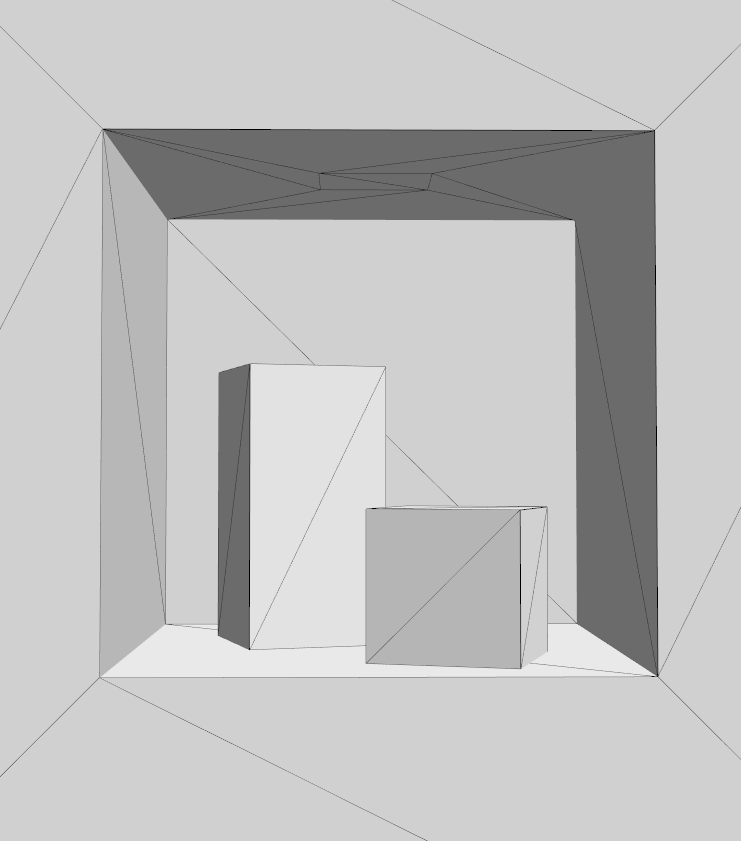
\includegraphics[width=0.65\textwidth]{Figures/editor/panels/VtkNavMode.png}
  \bicaption{三维场景视口：导航模式下的几何体可视化}{3D scene viewport: geometry visualization in navigation mode}
  \label{fig:gui:viewport}
\end{figure}

\subsection{交互式表面区域标注}
\label{sec:gui:painter}

如 \ref{sec:gui:dsl} 所述，DSL 的 $\langle\text{boundary-condition}\rangle$ 产生式要求每条边界条件通过 $\langle\text{triangles}\rangle$ 引用预先分割好的 STL 文件。当同一几何体表面需要划分为多个具有不同换热参数的子区域时，用户必须借助外部三维建模工具切割 STL 并分别导出。本模块（\texttt{SurfacePainter}）通过交互式画笔标注扩展了 DSL 在表面分区方面的能力——标注结果由写出器自动导出为独立 STL 文件并以 $\langle\text{stl-path}\rangle$ 引用，对求解器透明。

\subsubsection{数据结构}

\texttt{SurfacePainter} 在目标介质体的 \texttt{vtkPolyData} 单元数据中附加 \texttt{vtkIntArray}（字段名 \texttt{BoundaryLabel}），记录每个三角面片的区域归属编号（零值表示未归属）。每个面片至多属于一个 \texttt{SurfaceZone}，赋标签时自动从其他区域移除。

\subsubsection{标注操作}

画笔模式下使用 \texttt{vtkHardwareSelector} 执行矩形区域硬件拾取——在拾取通道中以颜色编码渲染场景，通过帧缓冲区获取目标矩形内命中的 Cell ID。提供四种标注操作：
\begin{itemize}
  \item \texttt{BRUSH}（画刷）：屏幕空间拖拽画刷，批量拾取并赋标签；
  \item \texttt{FLOOD\_FILL}（洪泛填充）：从点击面片出发，沿共享边进行 BFS 扩展到连通区域；
  \item \texttt{FILL\_ALL}（全部填充）：将介质体全部面片赋给当前区域；
  \item \texttt{REPLACE\_FILL}（全局替换）：将与点击面片同标签的所有面片改为当前区域。
\end{itemize}

每次落笔前将当前标注数组深拷贝压入撤销栈（最大深度 50），支持完整的撤销/重做操作。

图~\ref{fig:gui:painter} 展示了画笔模式下的表面区域标注过程，不同颜色标识不同边界条件区域。

\begin{figure}[htbp]
  \centering
  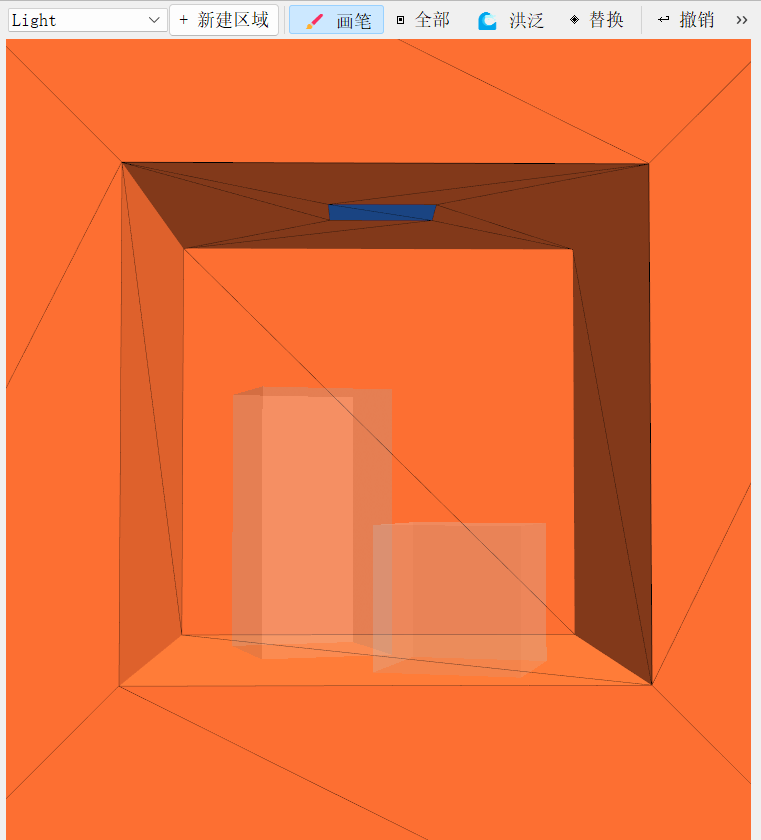
\includegraphics[width=0.65\textwidth]{Figures/editor/panels/VtkPaintMode.png}
  \bicaption{画笔模式下的交互式表面区域标注}{Interactive surface zone annotation in paint mode}
  \label{fig:gui:painter}
\end{figure}

\subsection{场景树与属性编辑}
\label{sec:gui:treeprop}

\texttt{SceneTreePanel} 以层级树形式投射语义模型的完整结构，树节点按类型分组：全局设置、几何体（各 \texttt{Body} 下挂载 \texttt{SurfaceZone}）、连接、探针、摄像机、光源和任务队列。表面区域节点按边界条件类型着色，便于快速识别 Dirichlet/Robin/Neumann/混合边界的分布。

\texttt{PropertyPanel} 根据当前选中节点类型动态切换对应属性编辑器：
\begin{itemize}
  \item \texttt{BodyEditor}：编辑 DSL $\langle\text{medium}\rangle$ 产生式的全部参数——介质类型、$\lambda$、$\rho$、$c_p$、$\delta$、$T_{\rm init}$、$T_{\rm imposed}$、体积热源功率、$\langle\text{side-specifier}\rangle$，以及该介质体的表面区域列表；
  \item \texttt{SurfaceZoneEditor}：编辑 DSL $\langle\text{boundary-condition}\rangle$ 各展开式的参数——Dirichlet 型（$T$）、Robin 型（$T_{\rm ref}$、$\varepsilon$、$f_s$、$h_c$、$T_{\rm env}$）、Neumann 型（$\Phi$）和混合型；
  \item \texttt{ConnectionEditor}：编辑 DSL $\langle\text{connection}\rangle$ 的参数（固-流连接或固-固连接的接触热阻）；
  \item \texttt{CameraEditor}、\texttt{ProbeEditor}、\texttt{LightEditor}：编辑 DSL 不涉及但仿真任务所需的场景对象（IR 摄像机位姿、探针坐标、灯光参数）。
\end{itemize}

属性编辑器的修改通过信号/槽链路写回 \texttt{SceneModel}，主窗口随后重建场景树并刷新视口。

图~\ref{fig:gui:treeprop} 展示了场景树与属性面板的联动界面，选中某一介质体时属性面板自动切换显示对应参数编辑器。

\begin{figure}[htbp]
  \centering
  \begin{subcaptiongroup}
  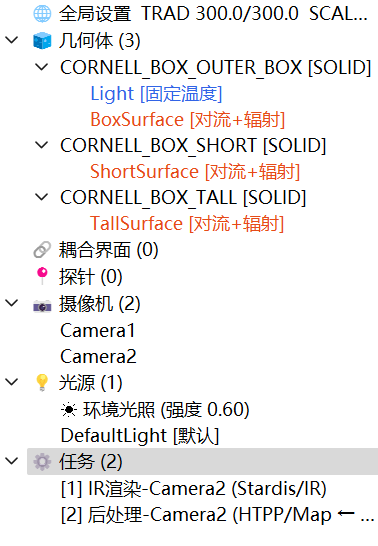
\includegraphics[height=0.42\textheight]{Figures/editor/panels/SceneTree.png}
  \hfill
  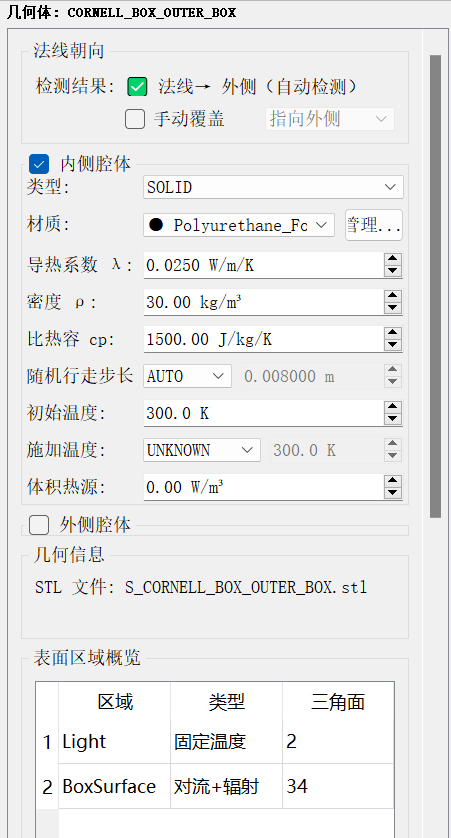
\includegraphics[height=0.42\textheight]{Figures/editor/panels/GeometryMeshConfig.png}
  \end{subcaptiongroup}
  \bicaption{场景树（左）与几何体属性编辑面板（右）}{Scene tree (left) and geometry property editor panel (right)}
  \label{fig:gui:treeprop}
\end{figure}

\subsection{仿真任务配置与执行}
\label{sec:gui:taskrunner}

Stardis CLI 的运行时参数（采样数、渲染分辨率、探针坐标等）和后处理工具 HTPP 的参数均不属于 \texttt{stardis-input} DSL 的定义范围。本模块将这些运行时参数结构化管理，以图形化界面替代手动命令行拼接。

\texttt{CommandBuilder} 将 \texttt{Task} 数据对象转换为可执行的 CLI 参数列表。任务通过名称引用 \texttt{SceneModel} 中的场景对象（如摄像机名称、探针名称列表），而非硬编码路径和数值。执行前由 \texttt{resolve\_all()} 将名称引用求值为实际 CLI 参数，确保场景编辑后重新执行时始终使用最新数据。HTPP 任务的输入文件同样通过引用队列中的 Stardis 任务输出来解析，避免硬编码路径。

\texttt{TaskRunner} 以 PyQt5 \texttt{QProcess} 管理子进程生命周期，在主线程事件循环中通过信号接收进程输出，日志面板实时更新。队列中的任务顺序执行；任务异常退出时按错误策略自动重试、跳过或暂停等待用户介入。

编辑器的偏好设置中，用户可将多个 Stardis/HTPP 可执行文件路径命名为标签（如 \texttt{CPU-Release}、\texttt{GPU-Release}），任务配置通过标签名引用——同一任务配置可通过切换标签在不同求解器版本间切换，直接对应第三、四章实验中的 CPU 基线与 GPU 加速版本选择。

图~\ref{fig:gui:taskrunner} 展示了任务配置与执行界面。左图为 Stardis IR 渲染任务的参数配置面板，设定了线程数、传导算法和摄像机引用等运行参数；中图为 IR 摄像机参数面板，设定了位姿、视场角、每像素采样数（SPP）和分辨率——IR 渲染模式下，图像分辨率与采样数由摄像机参数决定，而非任务面板中的样本数字段；右图为任务队列面板与实时运行日志。

\begin{figure}[htbp]
  \centering
  \begin{subcaptiongroup}
  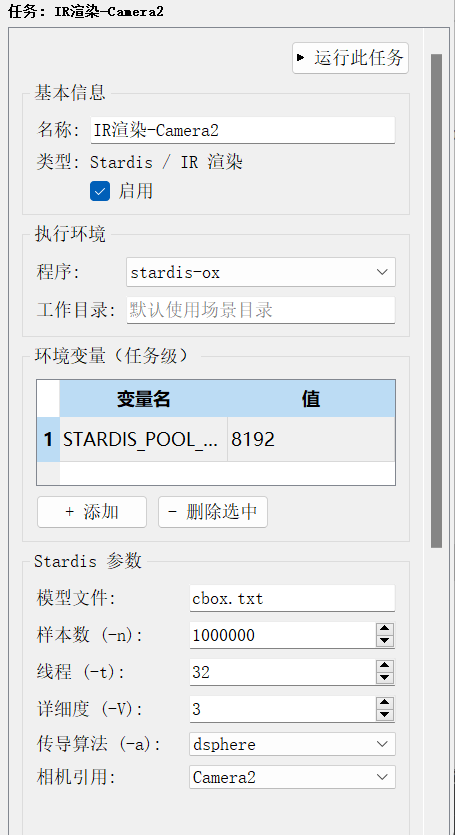
\includegraphics[height=0.4\textheight]{Figures/editor/panels/StardisConfig.png}
  \hfill
  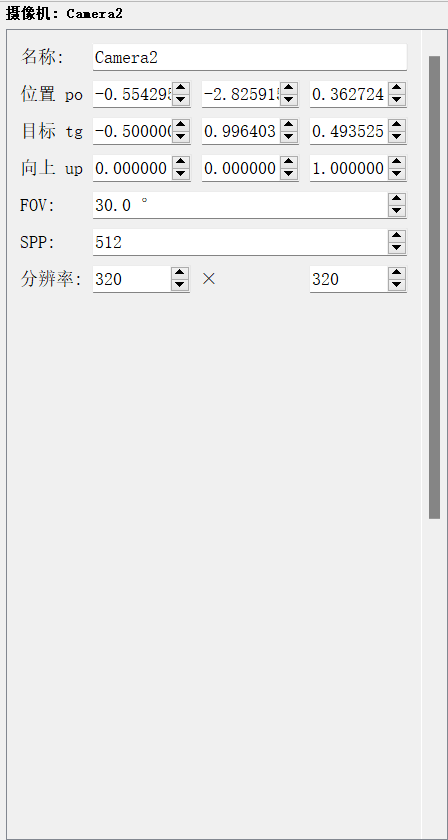
\includegraphics[height=0.4\textheight]{Figures/editor/panels/CameraConfig.png}
  \hfill
  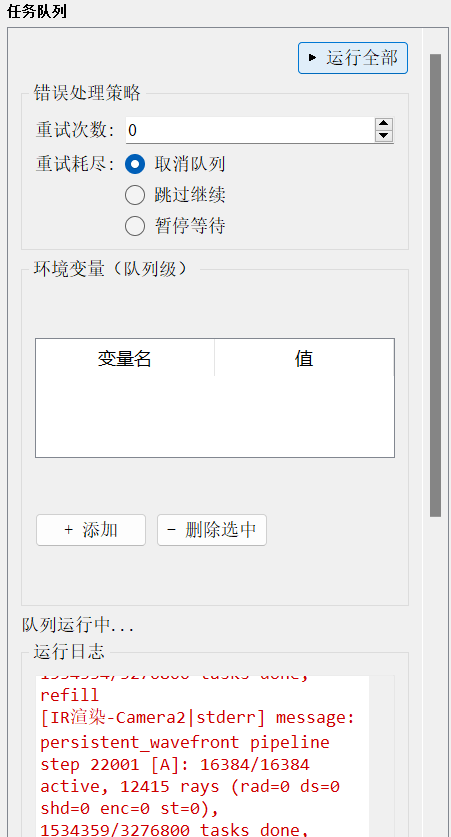
\includegraphics[height=0.4\textheight]{Figures/editor/panels/TaskQueue.png}
  \end{subcaptiongroup}
  \bicaption{Stardis 任务配置与执行界面}{Stardis task configuration and execution interface}
  \label{fig:gui:taskrunner}

  \small
  任务配置面板（左）、IR 摄像机参数面板（中）与任务队列面板（右）。
\end{figure}


%% ============================================================
\section{应用案例}
\label{sec:gui:cases}

本节以 Cornell Box 热仿真场景为例，演示从几何导入到仿真结果的完整工作流。经典 Cornell Box 场景以封闭空腔与内部几何体构成多次反射环境，广泛用于全局光照算法验证；类似地，本场景呈现多个导热体在封闭空间内，受顶部定温热源的辐射照射，在辐射、传导和对流三种耦合热输运过程共同作用下，达到稳态热平衡的红外仿真结果。

\subsection{场景描述}

场景包含三个 SOLID 介质体（图~\ref{fig:gui:case-import}）：外层盒体 \texttt{CORNELL\_BOX\_OUTER}（36 个三角面片）及内部两个长方体 \texttt{CORNELL\_BOX\_SHORT}（12 面片）和 \texttt{CORNELL\_BOX\_TALL}（12 面片），三者均以聚氨酯泡沫（Polyurethane Foam，$\lambda = 0.025\;\text{W/(m·K)}$，$\rho = 30\;\text{kg/m}^3$，$c_p = 1500\;\text{J/(kg·K)}$）为介质材料，初始温度 $T_{\rm init} = 300\;\text{K}$。

\begin{figure}[htbp]
  \centering
  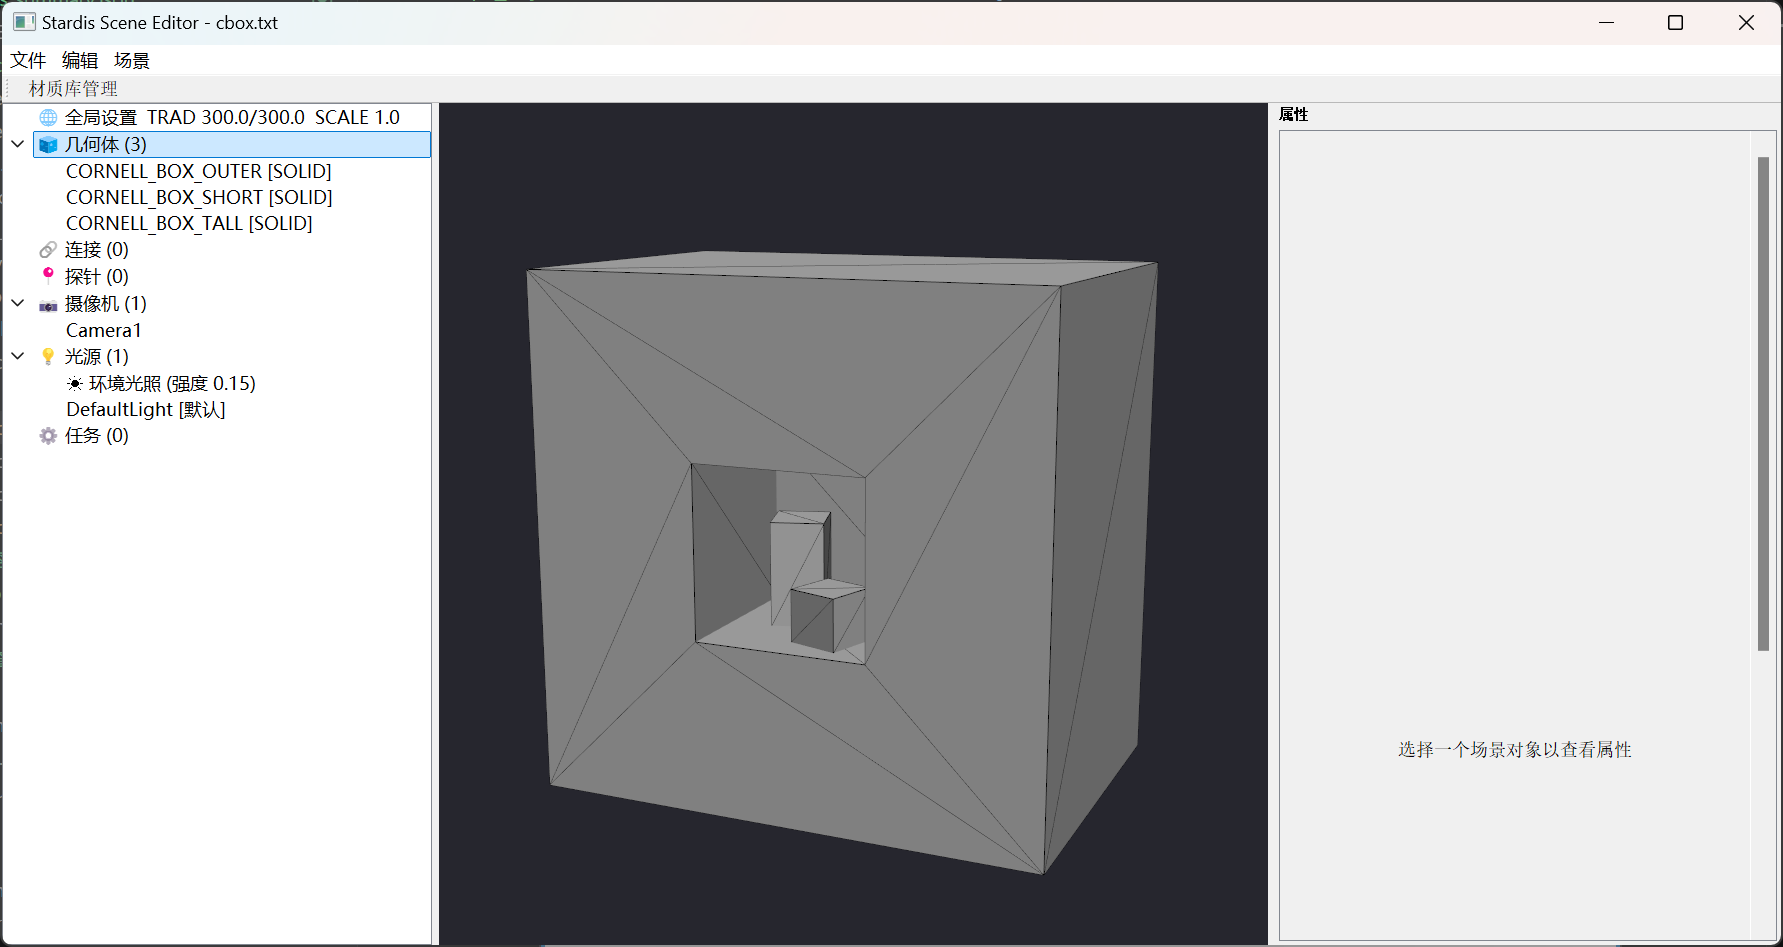
\includegraphics[width=0.85\textwidth]{Figures/editor/workflow/1_2_ImportedGeometry.png}
  \bicaption{Cornell Box 场景几何导入结果：三个 SOLID 介质体}{Cornell Box scene after geometry import: three SOLID media bodies}
  \label{fig:gui:case-import}
\end{figure}

\subsection{边界条件标注与任务配置}

利用画笔标注模块（\ref{sec:gui:painter}），在外层盒体表面划分两个边界条件区域：顶部 2 个面片标注为 \texttt{Light}（Dirichlet 型，$T = 1000\;\text{K}$），代表定温热源；其余 34 个面片标注为 \texttt{BoxSurface}（Robin 型，$\varepsilon = 0.9$，$h_c = 10\;\text{W/(m}^2\text{·K)}$，$T_{\rm env} = 300\;\text{K}$），代表与外部环境的对流-辐射耦合换热。两个内部长方体表面分别整体标注为 \texttt{ShortSurface} 和 \texttt{TallSurface}，边界条件类型与外壁相同。标注完成后，画笔模块自动为每个区域导出独立的 STL 文件供求解器引用。

图~\ref{fig:gui:case-paint-config} 展示了画笔标注与任务配置。左图为外层盒体的画笔标注结果，橙色区域为具有对流-辐射耦合换热的一般固体表面（\texttt{BoxSurface}，Robin 型，$\varepsilon = 0.9$，$h_c = 10\;\text{W/(m}^2\text{·K)}$），蓝色面片为顶部热源区域（\texttt{Light}，Dirichlet 型，$T = 1000\;\text{K}$）；右图为 Stardis IR 渲染任务的参数配置，设定了 32 线程、\texttt{dsphere} 传导算法，并通过 Camera2 的名称引用自动获取摄像机位姿与渲染参数（位姿、SPP、分辨率等，见图~\ref{fig:gui:taskrunner} 中图）。

\begin{figure}[htbp]
  \centering
  \begin{subcaptiongroup}
  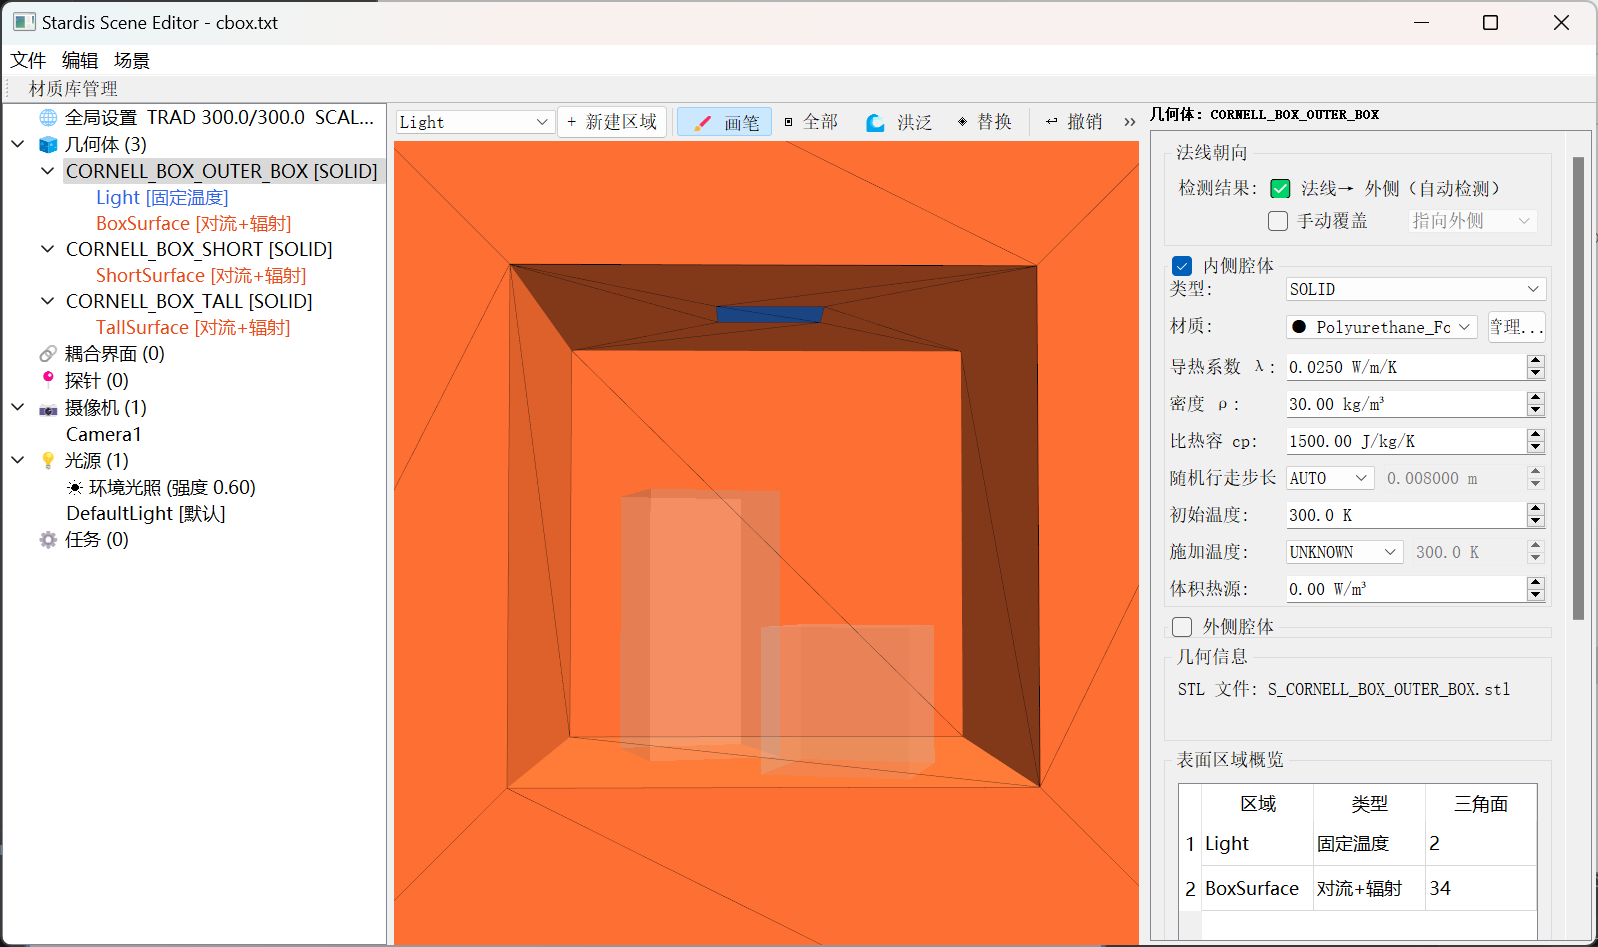
\includegraphics[width=0.48\textwidth]{Figures/editor/workflow/3_1_PaintBNDCondition.png}
  \hfill
  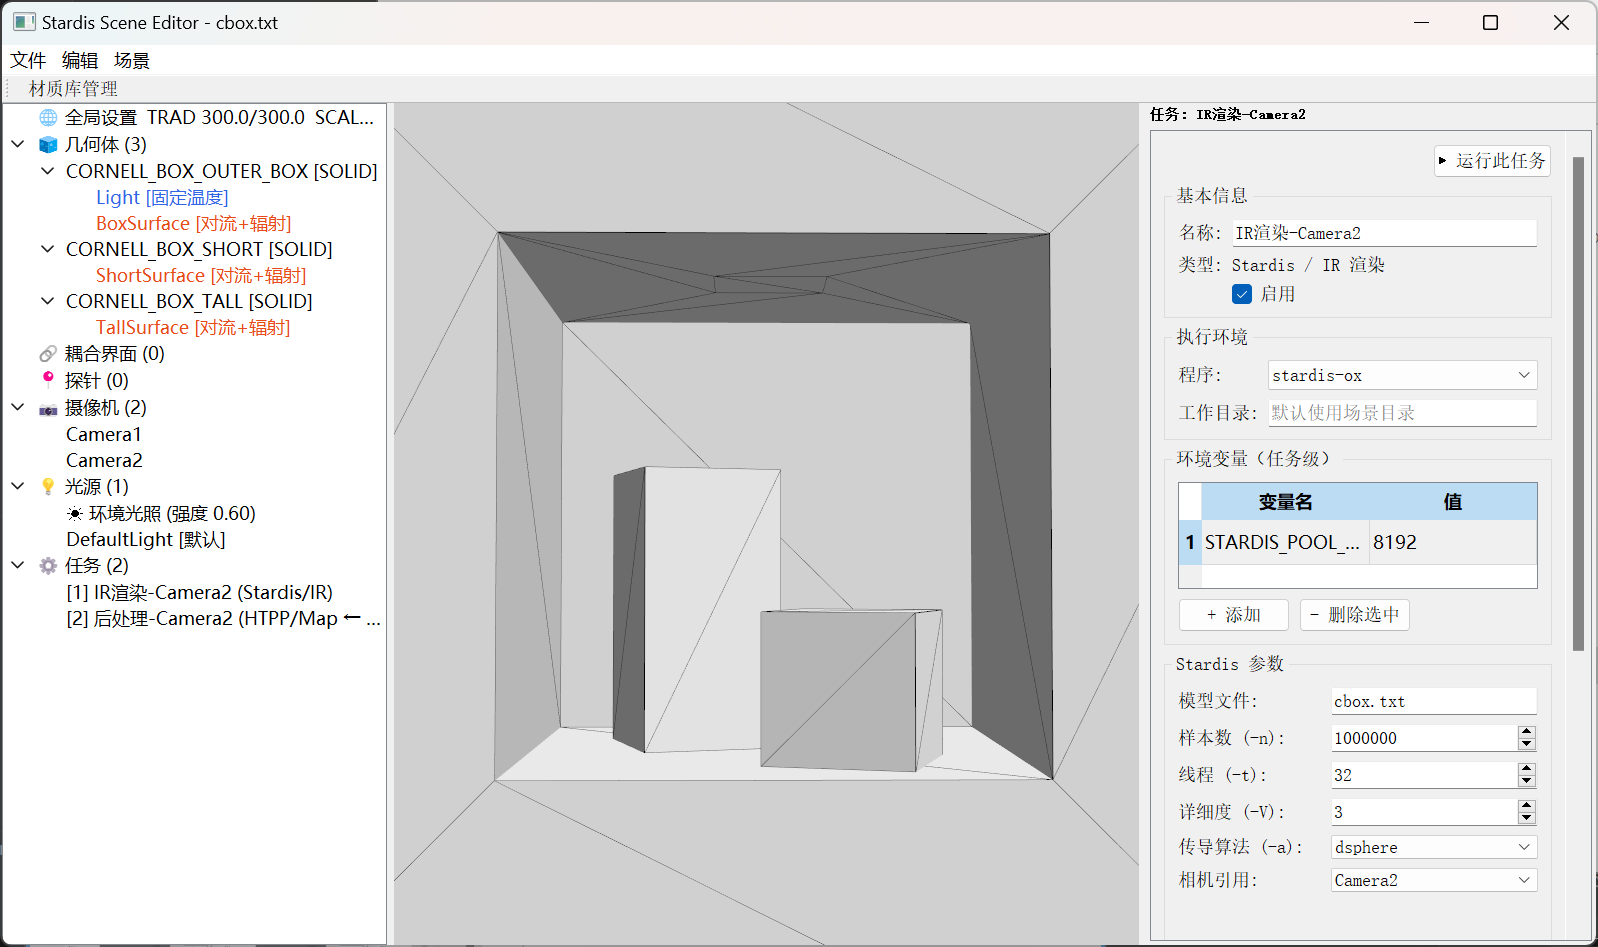
\includegraphics[width=0.48\textwidth]{Figures/editor/workflow/6_1_ConfigTask.png}
  \end{subcaptiongroup}
  \bicaption{外层盒体画笔标注（左）与 Stardis IR 渲染任务配置（右）}{Outer box boundary annotation (left) and Stardis IR rendering task configuration (right)}
  \label{fig:gui:case-paint-config}
\end{figure}

\subsection{仿真执行与结果}

任务队列依次执行 Stardis IR 渲染和 HTPP 后处理（色调映射）。运行日志面板实时显示 Wavefront 管线的迭代进度（如 \texttt{step 22001, 16384/16384 active}）。图~\ref{fig:gui:case-result} 为稳态热平衡下的红外仿真结果：顶部热源（$1000\;\text{K}$）呈高亮，盒体内壁因多次辐射反射和传导扩散产生连续温度梯度，两个内部长方体因较低导热系数呈现明显低温区域，整体温度场分布符合辐射-传导-对流耦合输运的物理预期。

\begin{figure}[htbp]
  \centering
  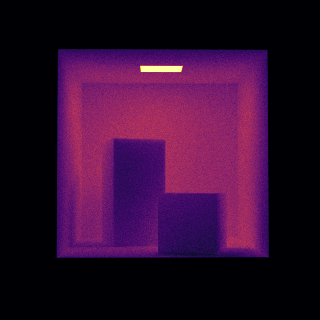
\includegraphics[width=0.45\textwidth]{Figures/editor/workflow/8_Result.png}
  \bicaption{Cornell Box 稳态红外仿真结果（inferno 色调映射）}{Cornell Box steady-state IR simulation result (inferno colormap)}
  \label{fig:gui:case-result}
\end{figure}

该案例展示了从 DSL 场景构建到红外仿真输出的完整闭环：几何导入与三维预览验证空间关系 → 画笔标注划分边界条件区域 → 属性编辑设定物理参数 → 任务配置引用场景对象 → 队列化执行与实时日志监控 → 后处理色调映射可视化。全部操作在 StardisEditor 内完成，无需手动编辑 DSL 文本或拼接命令行参数。

%% ============================================================
\section{小结}
\label{sec:gui:summary}

本章以 \texttt{stardis-input} 领域描述语言的形式文法为基础，设计并实现了 GUI 场景编辑器 StardisEditor。在 DSL 工具链层面，编辑器实现了语法感知的解析与写出闭环——\texttt{SceneParser} 按 BNF 文法将 DSL 文本解析为类型化语义模型 \texttt{SceneModel}，\texttt{SceneWriter} 将编辑后的模型序列化回合法 DSL 文本，包括将画笔标注的扩展语义自动映射为标准 STL 引用。在 DSL 表达能力之外，编辑器提供了三项关键扩展：基于 VTK 的三维几何可视化使空间关系和法线朝向直观可见；交互式画笔标注使表面区域划分无需借助外部建模工具；结构化任务配置与队列化执行替代了手动命令行拼接。可执行文件标签引用机制使任务配置在求解器版本管理层面联通了第三章 Wavefront 求解器和第四章 OptiX 后端的对比实验场景。

至此，论文完成了 Wavefront 并行化求解器（第三章）、OptiX GPU 光追后端（第四章）和场景编辑器（本章）三个核心贡献的阐述；第六章将对全文研究工作进行总结并展望未来研究方向。
